We looked at the one instance of knowledge-guided reasoning as semantic parsing in
Chapter~\ref{chapter:wikitables}. There we exploited the knowledge of the syntactic
and semantic properties of the target language to define a grammar that can
constrain the output space in an encoder-decoder model, thereby improving its
performance at question-answering on a hard reasoning task. While the training setup we
used there was weakly-supervised, and did not assume availability of annotated
logical forms, we still had to rely on a \emph{good} set of approximate
logical fnorms. In this chapter, we further relax the reliance on supervision,
and leverage more contextual knowledge to build a semantic parser from
question-answer pairs alone.

As we explained in Chapter~\ref{chapter:reasoning_related_work},  training
semantic parsers from question-answer pairs typically involves
searching over an exponentially large space of logical forms. Neural semantic
parsers do not include lexicons to provide guidance during search like their
traditional variants did, and thus have no way of differentiating paths leading
to correct logical forms from those that lead to spurious ones coincidentally
evaluating to the correct answers. To deal with this issue, we propose a search
process in this chapter that maximizes the relevance of the retrieved logical forms to the input
utterances through a learned lexical mapping, and a novel EM-like iterative
training algorithm that alternates between searching for consistent logical
forms and maximizing the marginal likelihood of the retrieved ones, with the
parameters from the maximization step being used to warm-start the search step
in the next iteration.

We demonstrate the effectiveness of these two techniques on two difficult
reasoning tasks: \WTQ{}(WTQ)~\citep{pasupat2015compositional}, an open domain
task with significant lexical variation, and Cornell Natural Language Visual
Reasoning (NLVR)~\citep{suhr2017corpus}, a closed domain task with binary
denotations, and thus far less supervision. We show that: 1) interleaving
online search and MML over retrieved logical forms
(Section~\ref{sec:iterative_search}) is a more effective training algorithm than each
of those objectives alone; 2) coverage guidance during search
(Section~\ref{sec:coverage_guided_search}) is helpful for dealing with weak
supervision, more so in the case of NLVR where the supervision is weaker; 3) a
combination of the two techniques yields $44.3\%$ test accuracy on WTQ,
outperforming the previous best single model in a comparable setting, and
$82.9\%$ test accuracy on NLVR, outperforming the best prior model, which also
relies on greater supervision.

\section{Coverage-guided search}\label{sec:coverage_guided_search}
Weakly-supervised training of semantic parsers relies heavily on lexical cues
to guide the initial stages of learning to good logical forms.  Traditionally,
these lexical cues were provided in the parser's lexicon.  Neural semantic
parsers remove the lexicon, however, and so need another mechanism for
obtaining these lexical cues.  In this section we introduce the use of coverage
to inject lexicon-like information into neural semantic parsers.

Coverage is a measure of relevance of the candidate logical form $y_i$ to the
input $x_i$, in terms of how well the productions in $y_i$ map to parts of
$x_i$. We use a small manually specified lexicon as a mapping from source
language to the target language productions, and define coverage of $y_i$ as
the number of productions triggered by the input utterance, according to the
lexicon, that are included in $y_i$.

We use this measure of coverage to augment our loss function, and train using
an MBR based algorithm as follows. We use beam search to train a model to
minimize the expected value of a cost function $\mathcal{C}$: \begin{equation}
	\min_{\theta} \sum_{i=1}^{N} \mathbb{E}_{\tilde{p}(y_i|x_i;
	\theta)}\mathcal{C}(x_i, y_i, w_i, d_i) \label{eq:erm} \end{equation}

\noindent where $\tilde{p}$ is a \emph{re-normalization}\footnote{Note that
without this re-normalization, and with a -1/0 cost function based on
denotation accuracy, MBR will maximize the likelihood of correct logical forms
on the beam, which is equivalent to dynamic MML.} of the probabilities assigned
to all logical forms on the beam.

We define the cost function $\mathcal{C}$ as: \begin{equation} \mathcal{C}(x_i,
y_i, w_i, d_i) = \lambda \mathcal{S}(y_i, x_i) + \\ (1 -
\lambda)\mathcal{T}(y_i, w_i, d_i) \label{eq:cost} \end{equation} where the
function $\mathcal{S}$ measures the number of items that $y_i$ is missing from
the actions (or grammar production rules) triggered by the input utterance
$x_i$ given the lexicon; and the function $\mathcal{T}$ measures the
consistency of the evaluation of $y_i$ in $w_i$, meaning that it is $0$ if
$\llbracket y_i\rrbracket^{w_i} = d_i$, or a value $e$ otherwise.  We set $e$
as the maximum possible value of the coverage cost for the corresponding
instance, to make the two costs comparable in magnitude.  $\lambda$ is a
hyperparameter that gives the relative weight of the coverage cost.


\section{Iterative search} \label{sec:iterative_search} In this section we
describe the iterative technique for refining the set of candidate logical
forms associated with each training instance.

As discussed in \secref{sec:weak_supervision} in Chapter~\ref{chapter:reasoning_related_work},
most prior work on
weakly-supervised training of semantic parsers uses dynamic MML.  This is
particularly problematic in domains like NLVR, where the supervision signal is
binary---it is very hard for dynamic MML to bootstrap its way to finding good
logical forms.  To solve this problem, we interleave static MML, which has a
consistent supervision signal from the start of training, with the
coverage-augmented MBR algorithm described
in~\secref{sec:coverage_guided_search}.

In order to use static MML, we need an initial set of candidate logical forms.
We obtain this candidate set using a bounded-length exhaustive search, filtered
using heuristics based on the same lexical mapping used for coverage
in~\secref{sec:coverage_guided_search}.  A bounded-length search will not find
logical forms for the entire training data, so we can only use a subset of the
data for initial training.  We train a model to convergence using static MML on
these logical forms, then use that model to initialize coverage-augmented MBR
training.  This gives the model a good starting place for the dynamic learning
algorithm, and the search at training time can look for logical forms that are
longer than could be found with the bounded-length exhaustive search.  We train
MBR to convergence, then use beam search on the MBR model to find a new set of
candidate logical forms for static MML on the training data.  This set of
logical forms can have a greater length than those in the initial set, because
this search uses model scores to not exhaustively explore all possible paths,
and thus will likely cover more of the training data.  In this way, we can
iteratively improve the candidate logical forms used for static training, which
in turn improves the starting place for the online search algorithm.

\begin{algorithm} \SetAlgoLined \SetKwInOut{Input}{Input}
	\SetKwInOut{Output}{Output} \Input{Dataset $\mathcal{D} = \{X, W, D\}$;
	and \\ seed set $\mathcal{D}^0 = \{X^0, Y^0\}$ such that \\ $X^0
	\subset X$ and $\mathcal{C}(x^0_i, y^0_i, W_i, D_i) =0$} \Output{Model
	parameters $\theta^{\texttt{MBR}}$} Initialize dataset
	$\mathcal{D}^{\texttt{MML}} = \mathcal{D}^0$\;
	\While{$\text{Acc}(\mathcal{D}_{\text{dev}})$ is increasing}{
		$\theta^{\texttt{MML}} =
		\texttt{MML}(\mathcal{D}^{\texttt{MML}})$\; Initialize
		$\theta^{\texttt{MBR}} = \theta^{\texttt{MML}}$\; Update
		$\theta^{\texttt{MBR}} = \texttt{MBR}(\mathcal{D};
		\theta^{\texttt{MBR}})$\; Update $\mathcal{D}^{\texttt{MML}} =
		\texttt{Decode}(\mathcal{D}; \theta^{\texttt{MBR}})$\; }
\caption{Iterative coverage-guided search} \label{alg:iterative_search}
\end{algorithm}

Algorithm~\ref{alg:iterative_search} concretely describes this process.
\texttt{Decode} in the algorithm refers to running a beam search decoder that
returns a set of consistent logical forms (i.e. $\mathcal{T} = 0$) for each of
the input utterances. We start off with a seed dataset $\mathcal{D}^0$ for
which consistent logical forms are available.

\section{Task Details} \label{sec:datasets}
We already described \WTQ{} in
Chapter~\ref{chapter:wikitables}.
We will now describe the NLVR dataset in greater detail.

Cornell NLVR is a language-grounding dataset containing natural language
sentences provided along with synthetically generated visual contexts, and a
label for each sentence-image pair indicating whether the sentence is true or
false in the given context.
\begin{figure} \centering
	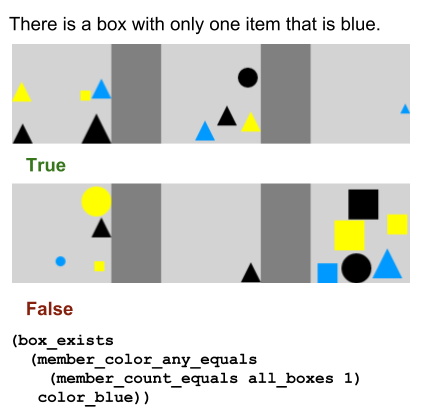
\includegraphics[width=4in]{figures/nlvr_example_with_worlds_and_lf.png}
	\caption{Example
	from NLVR dataset showing one sentence associated with two worlds and
	corresponding binary labels, and translation of the sentence above in
	our logical form language. Also shown are the actions triggered by the lexicon from the utterance} \label{fig:nlvr_example_with_two_worlds} 
\end{figure}
Figure~\ref{fig:nlvr_example_with_two_worlds} shows two example sentence-image pairs
from the dataset (with the same sentence). The dataset also comes with
structured representations of images, indicating the color, shape, size,
and x- and y-coordinates of each of the objects in the image. While we
show images in Figure~\ref{fig:nlvr_example_with_two_worlds} for ease of exposition, we
use the structured representations in this work.

Recall the formal notation for semantic parsing we introduced in
Chapter~\ref{chapter:reasoning_related_work},
Section~\ref{sec:semantic_parsing_formal_definition}. There we identified that
the dataset during training in a weakly supervised setup is typically $\{x_i,
w_i, d_i\}_{i=1}^N$, where
each utterance $x_i$ comes with a world $w_i$, and the corresponding denotation
$d_i$. 
A special property of the NLVR dataset is that the same sentence occurs with
multiple worlds. While searching for logical forms that execute to a particular
denotation, either during training or otherwise, this property can be exploited
as follows: We can define a stricter objective that a logical form for a given
utterance must evaluate to the correct denotation (either \textit{True} or
\textit{False}) in \emph{all} the worlds it occurs in. We do this, as described
in Section~\ref{sec:coverage_guided_search}. Accordingly, we tweak the general
notation for semantic parsing problems as follows: We define the dataset as
$\{x_i, W_i, D_i\}_{i=1}^N$, where $W_i = \{w_i^j\}_{j=1}^M$ is the set of all
the worlds that $x_i$ occurs in, and $D_i = \{d_i^j\}_{j=1}^M$ is the set of
corresponding denotations.

Going back to Figure~\ref{fig:nlvr_example_with_two_worlds},
$x_i$ is \textit{There is a box with only one item that is blue}, the structured
representations associated with the two images shown are two of the worlds
($w^1_i$ and $w^2_i$), in which a translation of the utterance in some logical form
language could be evaluated. The corresponding labels, \textit{True} and
\textit{False} respectively, are the denotations $d^1_i$ and $d^2_i$ that 
the translation is supposed to produce, when executed in the two worlds
respectively. Figure~\ref{fig:nlvr_example_with_two_worlds} also shows such a
translated logical form, written in the language we will describe next.

\subsection{Logical form languages} \label{sec:logical_form_languages}
\subsubsection{NLVR}
For NLVR, we define a typed variable-free functional query language, inspired by the
GeoQuery language \citep{zelle1996learning}. Our language contains six basic
types: \texttt{box} (referring to one of the three gray areas in
Figure~\ref{fig:nlvr_example_with_two_worlds}), \texttt{object} (referring to the circles,
triangles and squares in Figure~\ref{fig:nlvr_example_with_two_worlds}), \texttt{shape},
\texttt{color}, \texttt{number} and \texttt{boolean}. The constants in our
language are color and shape names, the set of all boxes in an image, and the
set of all objects in an image. The functions in our language include those for
filtering objects and boxes, and making assertions, a higher order function for
handling negations, and a function for querying objects in boxes. This type
specification of constants and functions gives us a grammar with 115
productions, of which 101 are terminal productions.
(see Figure~\ref{fig:nlvr_grammar}
for the complete set of rules in our grammar).
Figure~\ref{fig:nlvr_example_with_two_worlds} shows an example of a complete logical form in our language.

\begin{figure}
	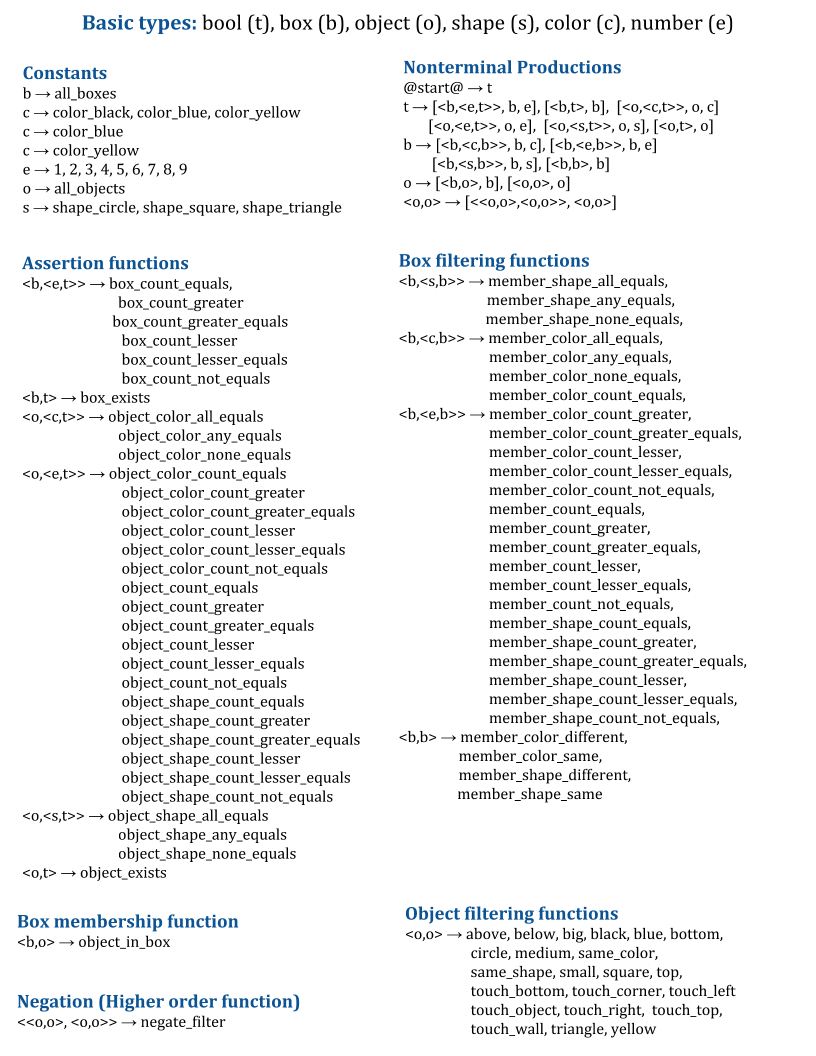
\includegraphics[width=\textwidth]{figures/nlvr_grammar.png}
	\caption{Complete grammar used by our parser for the NLVR
	domain}\label{fig:nlvr_grammar}
\end{figure}

\subsubsection{\WTQ{}}
\begin{figure}
    \centering
    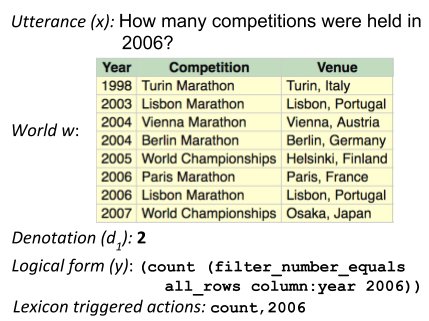
\includegraphics[width=3.5in]{figures/wtq_example_with_var_free_lang.png}
    \caption{Example from \WTQ{} dataset showing an utterance, a world, associated denotation, corresponding logical form, and actions triggered by the lexicon.}
    \label{fig:wtq_example_with_mapo_lang}
\end{figure}
For \WTQ{} we use the language presented in~\cite{liang2018memory}. This is a
variable-free language as well. We use this language instead of $\lambda$-DCS,
like we did in Chapter~\ref{chapter:wikitables}, because we found that the
logical forms produced by the variable free language are on average shorter than
the $\lambda$-DCS ones, which makes the former a good choice for our learning
algorithm in this chapter. The lack of variables makes this new language less
expressive than $\lambda$-DCS, but we actually found that to be helpful in
avoiding spurious logical forms to some extent. Figure~\ref{fig:wtq_example_with_mapo_lang}
shows an example of a context and a question from~\WTQ{}, along with an associated
logical form from the language defined by~\cite{liang2018memory}.

\subsection{Lexicons for coverage}\label{sec:coverage_lexicon} The lexicon we
use for the coverage measure described in~\secref{sec:coverage_guided_search}
contains under 40 rules for each logical form language. They mainly map words
and phrases to constants and unary functions in the target language. The
complete lexicons are shown in Tables~\ref{tab:nlvr_lexicon} and~\ref{tab:wtq_lexicon}.
Table~\ref{tab:nlvr_lexicon} uses the following placeholders:
\begin{align*}
    &\texttt{color} \in \{\texttt{yellow}, \texttt{blue}, \texttt{black}\}\\
    &\texttt{shape} \in \{\texttt{square}, \texttt{triangle}, \texttt{circle}\}\\
    &\texttt{size} \in \{\texttt{big}, \texttt{medium}, \texttt{small}\}\\
    &\texttt{location} \in \{\texttt{above}, \texttt{below}, \texttt{top}, \texttt{left},\\ 
    &\hspace{1em}\texttt{right},\texttt{bottom}, \texttt{corner}, \texttt{wall}\}\\
    &\texttt{number} \in \{1...9\}
\end{align*}

Figures~\ref{fig:nlvr_example_with_two_worlds}
and~\ref{fig:wtq_example_with_mapo_lang} also show the actions triggered by the corresponding
lexicons for the utterances shown. We find that small but precise lexicons are
sufficient to guide the search process away from spurious logical forms.
Moreover, as shown empirically in \secref{sec:results_coverage}, the model for
NLVR does not learn much without this simple but crucial guidance.

\begin{table}
\begin{tabular}{l}
	there is a box $\rightarrow$ \texttt{box\_exists}\\
	there is a [other] $\rightarrow$ \texttt{object\_exists}\\
	box $\ldots$ [color] $\rightarrow$ \texttt{color\_[color]}\\
	box $\ldots$ [shape] $\rightarrow$ \texttt{shape\_[shape]}\\
	not $\rightarrow$ \texttt{negate\_filter}\\
	contains $\rightarrow$ \texttt{object\_in\_box}\\
	touch $\ldots$ [location] $\rightarrow$ \texttt{touch\_[location]}\\
	\text{[location]} $\rightarrow$ \texttt{[location]}\\
	\text{[shape]} $\rightarrow$ \texttt{[shape]}\\
	\text{[color]} $\rightarrow$ \texttt{[color]}\\
	\text{[size]} $\rightarrow$ \texttt{[size]}\\
	\text{[number]} $\rightarrow$ \texttt{[number]}
\end{tabular}
\caption{Coverage Lexicon for NLVR}\label{tab:nlvr_lexicon}
\end{table}

\begin{table}
\begin{tabular}{l}
	at least $\rightarrow$ $\texttt{filter}_{\geq}$\\
	\text{[greater\textbar larger\textbar more] than} $\rightarrow$ $\texttt{filter}_{\geq}$ \\ 
	at most $\rightarrow$ $\texttt{filter}_{\leq}$\\
	\text{no [greater\textbar larger\textbar more] than} $\rightarrow$ $\texttt{filter}_{\leq}$ \\
	\text{[next\textbar below\textbar after]} $\rightarrow$ \texttt{next} \\
	\text{[previous\textbar above\textbar before]} $\rightarrow$ \texttt{previous} \\
	\text{[first\textbar top]} $\rightarrow$ \texttt{top} \\
	\text{[last\textbar bottom]} $\rightarrow$ \texttt{bottom} \\
	\text{same} $\rightarrow$ \texttt{same\_as} \\
	\text{total} $\rightarrow$ \texttt{sum} \\
	\text{difference} $\rightarrow$ \texttt{diff} \\
	\text{average} $\rightarrow$ \texttt{average} \\
	\text{[least\textbar smallest\textbar lowest\textbar smallest]} $\rightarrow$ \texttt{argmin} \\
	\text{[most\textbar longest\textbar highest\textbar largest]} $\rightarrow$ \texttt{argmax} \\
	\text{[what\textbar when]} $\ldots$ [last\text{\textbar}least] $\rightarrow$ \texttt{min} \\
	\text{[what\textbar when]} $\ldots$ [first\text{\textbar}most] $\rightarrow$ \texttt{max} \\
	\text{how many} $\rightarrow$ \texttt{count}
\end{tabular}
\caption{Coverage Lexicon for \WTQ{}}\label{tab:wtq_lexicon}
\end{table}

\section{Experiments} \label{sec:experiments}

We evaluate both our contributions on NLVR and \WTQ{}.

\subsection{Model} \label{sec:type_constrained_decoding}
In this work, we use a grammar-constrained encoder-decoder neural semantic
parser for our experiments.  Of the many variants of this basic architecture,
all of which are essentially seq2seq models
with constrained outputs and/or re-parameterizations, we choose to use the
parser of \citet{krishnamurthy2017neural}, as it is particularly well-suited to
the \WTQ{} dataset, which we evaluate on.

The encoder in the model is a bi-directional recurrent neural network with Long
Short-Term Memory (LSTM) \citep{hochreiter1997long} cells, and the decoder is a
grammar-constrained decoder also with LSTM cells.  Instead of directly
outputting tokens in the logical form, the decoder outputs \emph{production
rules} from a CFG-like grammar.  These production rules sequentially build up
an abstract syntax tree, which determines the logical form.  The model also has
an entity linking component for producing table entities in the logical forms;
this component is only applicable to \WTQ{}, and we remove it when running
experiments on NLVR.  The particulars of the model are not the focus of this
work, so we refer the reader to the original paper for more details.

In addition, we slightly modify the constrained decoding architecture
from~\cite{krishnamurthy2017neural} to bias the predicted actions towards those
that would decrease the value of $\mathcal{S}(y_i, x_i)$. This is done using a
coverage vector, $v^{\mathcal{S}}_i$ for each training instance that keeps
track of the production rules triggered by $x_i$, and gets updated whenever one
of those desired productions is produced by the decoder. That is,
$v^{\mathcal{S}}_i$ is a vector of 1s and 0s, with 1s indicating the triggered
productions that are yet to be produced by the decoder. This is similar to the
idea of checklists used by \citet{kiddon2016globally}. The decoder in the
original architecture scores output actions at each time step by computing a
dot product of the predicted action representation with the embeddings of each
of the actions. We add a weighted sum of all the actions that are yet to
produced: \begin{equation} s^a_i = e^a . (p_i + \gamma * v^{\mathcal{S}}_i . E)
\end{equation} where $s^a_i$ is the score of action $a$ at time step $i$, $e^a$
is the embedding of that action, $p_i$ is the predicted action representation,
$E$ is the set of embeddings of all the actions, and $\gamma$ is a learned
parameter for regularizing the bias towards yet-to-be produced triggered
actions.

\subsection{Experimental setup}\label{sec:exp_setup}
\paragraph{NLVR} We use the standard train-dev-test split for NLVR, containing 12409, 988 and 989 sentence-image pairs respectively. NLVR contains most of the sentences occurring in multiple worlds (with an average of 3.9 worlds per sentence). We set the word embedding and action embedding sizes to 50, and the hidden layer size of both the encoder and the decoder to 30. We initialized all the parameters, including the word and action embeddings using Glorot uniform initialization \citep{glorot2010understanding}. We found that using pretrained word representations did not help. We added a dropout \citep{srivastava2014dropout} of 0.2 on the outputs of the encoder and the decoder and before predicting the next action, set the beam size to 10 both during training and at test time, and trained the model using ADAM \citep{kingma2014adam} with a learning rate of 0.001. All the hyper-parameters are tuned on the validation set. 


\paragraph{\WTQ} This dataset comes with five different cross-validation folds of training data, each containing a different 80/20 split for training and development. We first show results aggregated from all five folds in \secref{sec:main_results}, and then show results from controlled experiments on fold 1. We replicated the model presented in \citet{krishnamurthy2017neural}, and only changed the training algorithm and the language used. We used a beam size of 20 for MBR during training and decoding, and 10 for MML during decoding, and trained the model using Stochastic Gradient Descent~\citep{kiefer1952stochastic} with a learning rate of 0.1, all of which are tuned on the validation sets.

\paragraph{Specifics of iterative search} For our iterative search algorithm, we obtain an initial set of candidate logical forms in both domains by exhaustively searching to a depth of 10\footnote{It was prohibitively expensive to search beyond depth of 10.}. During search we retrieve the logical forms that lead to the correct denotations in all the corresponding worlds, and sort them based on their coverage cost using the coverage lexicon described in \secref{sec:coverage_lexicon}, and choose the top-$k$\footnote{$k$ is a hyperparameter that is chosen on the dev set at each iteration in iterative search, and is typically $10$ or $20$}. At each iteration of the search step in our iterative training algorithm, we increase the maximum depth of our search with a step-size of 2, finding more complex logical forms and covering a larger proportion of the training data. While exhaustive search is prohibitively expensive beyond a fixed number of steps, our training process that uses beam search based approximation can go deeper.

\paragraph{Implementation} We implemented our model and training algorithms within the AllenNLP \citep{Gardner2018AllenNLPAD} toolkit. The code and models are publicly available at \url{https://github.com/allenai/iterative-search-semparse}.

\subsection{Main results}\label{sec:main_results}
\paragraph{\WTQ{}}Table~\ref{tab:wtq_comparison} compares the performance of a single model trained using Iterative Search, with that of previously published single models. We excluded ensemble models since there are differences in the way ensembles are built for this task in previous work, either in terms of size or how the individual models were chosen. We show both best and average (over 5 folds) single model performance from \citet{liang2018memory} (Memory Augmented Policy Optimization). The best model was chosen based on performance on the development set. Our single model performances are computed in the same way. Note that \citet{liang2018memory} also use a lexicon similar to ours to prune the seed set of logical forms used to initialize their memory buffer.

In Table~\ref{tab:wtq_main_result}, we compare the performance of our iterative search algorithm with three baselines: 1) Static MML, as described in~\secref{sec:mml} trained on the candidate set of logical forms obtained through the heuristic search technique described in~\secref{sec:exp_setup}; 2) Iterative MML, also an iterative technique but unlike iterative search, we skip MBR and iteratively train static MML models while increasing the number of decoding steps; and 3) MAPO \citep{liang2018memory}, the current best published system on WTQ. All four algorithms are trained and evaluated on the first fold, use the same language, and the bottom three use the same model and the same set of logical forms used to train static MML.
\begin{table}
    \centering
    \begin{tabular}{lcc}
        \toprule
         \textbf{Approach} & \textbf{Dev} & \textbf{Test} \\
         \midrule
         \citet{pasupat2015compositional} & 37.0 & 37.1 \\
         \citet{neelakantan2016learning} & 34.1 & 34.2 \\
         \citet{Haug2018NeuralMR} & - & 34.8 \\
         \citet{zhang2017macro} & 40.4 & 43.7 \\
         \citet{liang2018memory} (MAPO) (mean $\pm$ std.) & 42.3 $\pm$ 0.3 & 43.1 $\pm$ 0.5 \\
         \citet{liang2018memory} (MAPO) (best) & 42.7 & 43.8 \\
         Iterative Search (mean $\pm$ std.) & 42.1 $\pm$ 1.1 & 43.9 $\pm$ 0.3 \\
         Iterative Search (best) & \textbf{43.1} & \textbf{44.3} \\
         \bottomrule
    \end{tabular}
    \caption{Comparison of single model performances of Iterative Search with previously reported single model performances}\label{tab:wtq_comparison}
\end{table}

\begin{table}
    \centering
    \begin{tabular}{lcc}
        \toprule
         \textbf{Algorithm} & \textbf{Dev acc.} & \textbf{Test acc.} \\
         \midrule
         MAPO & 42.1 & 42.7 \\
         \midrule
         Static MML & 40.0 & 42.2 \\
         Iterative MML & 42.5 & 43.1 \\
         Iterative Search & \textbf{43.0} & \textbf{43.8} \\
         \bottomrule
    \end{tabular}
    \caption{Comparison of iterative search with static MML, iterative MML, and the previous best result from~\cite{liang2018memory}, all trained on the official split 1 of \WTQ{} and tested on the official test set.}
    \label{tab:wtq_main_result}
\end{table}

\paragraph{NLVR} In Table~\ref{tab:main_result}, we show a comparison of the performance of our \textit{iterative coverage-guided search} algorithm with the previously published approaches for NLVR. The first two rows correspond to models that are not semantic parsers. This shows that semantic parsing is a promising direction for this task. The closest work to ours is the weakly supervised parser built by \cite{goldman2017weakly}. They build a lexicon similar to ours for mapping surface forms in input sentences to abstract clusters. But in addition to defining a lexicon, they also manually annotate complete sentences in this abstract space, and use those annotations to perform data augmentation for training a supervised parser, which is then used to initialize a weakly supervised parser. They also explicitly use the abstractions to augment the beam during decoding using caching, and a separately-trained discriminative re-ranker to re-order the logical forms on the beam.  As a discriminative re-ranker is orthogonal to our contributions, we show their results with and without it, with ``Abs. Sup.'' being more comparable to our work. Our model, which uses no data augmentation, no caching during decoding, and no discriminative re-ranker, outperforms their variant without reranking on the public test set, and outperforms their best model on the hidden test set, achieving a new state-of-the-art result on this dataset.

\begin{table*}
    \centering
    \begin{tabular}{lcccccc}
        \toprule
        \multicolumn{1}{c}{} & \multicolumn{2}{c}{\textbf{Dev.}} & \multicolumn{2}{c}{\textbf{Test-P}} & \multicolumn{2}{c}{\textbf{Test-H}} \\
        \textbf{Approach} & Acc. & Cons. & Acc. & Cons. & Acc. & Cons.\\
        \midrule
        MaxEnt \citep{suhr2017corpus} & 68.0 & - & 67.7 & - & 67.8 & - \\
        BiATT-Pointer \citep{tan2018object} & 74.6 & - & 73.9 & - & 71.8 & - \\
        Abs. Sup. \citep{goldman2017weakly} & 84.3 & 66.3 & 81.7 & 60.1 & - & - \\
        Abs. Sup. + ReRank \citep{goldman2017weakly} & 85.7 & 67.4 & 84.0 & 65.0 & 82.5 & 63.9 \\
        Iterative Search & 85.4 & 64.8 & 82.4 & 61.3 & \textbf{82.9} & \textbf{64.3} \\
        \bottomrule
    \end{tabular}
    \caption{Comparison of our approach with previously published approaches. We show accuracy and consistency on the development set, and public (Test-P) and hidden (Test-H) test sets.}
    \label{tab:main_result}
\end{table*}

\begin{table}
    \centering
    \begin{tabular}{lcccc}
        \toprule
        \multicolumn{1}{c}{}& \multicolumn{2}{c}{No coverage} & \multicolumn{2}{c}{+ coverage} \\
        \multicolumn{1}{c}{}& Acc. & Cons. & Acc. & Cons. \\
        \midrule
         No init.  & 56.4 & 12.0 & 73.9 & 43.6 \\
         MML init. & 77.7 & 51.1 & 80.7 & 56.4 \\
         \bottomrule
    \end{tabular}
    \caption{Effect of coverage guidance on NLVR parsers trained with and without initialization from an MML model. Metrics shown are accuracy and consistency on the public test set.}
    \label{tab:coverage_guidance}
\end{table}
\subsection{Effect of coverage-guided search} \label{sec:results_coverage}
To evaluate the contribution of coverage-guided search, we compare the the performance of the NLVR parser in two different settings: with and without coverage guidance in the cost function. We also compare the performance of the parser in the two settings, when initialized with parameters from an MML model trained to maximize the likelihood of the set of logical forms obtained from exhaustive search. Table~\ref{tab:coverage_guidance} shows the results of this comparison. We measure accuracy and consistency of all four models on the publicly available test set, using the official evaluation script. Consistency here refers to the percentage of logical forms that produce the correct denotation in all the corresponding worlds, and is hence a stricter metric than accuracy. The cost weight ($\lambda$ in Equation~\ref{eq:cost}) was tuned based on validation set performance for the runs with coverage, and we found that $\lambda = 0.4$ worked best.

It can be seen that both with and without initialization, coverage guidance helps by a big margin, with the gap being even more prominent in the case where there is no initialization. When there is neither coverage guidance nor a good initialization, the model does not learn much from unguided search and get a test accuracy not much higher than the majority baseline of 56.2\%.

We found that coverage guidance was not as useful for WTQ. The average value of the best performing $\lambda$ was around $0.2$, and higher values neither helped nor hurt performance.  

\begin{table}
    \centering
    \begin{tabular}{lllcc}
    \toprule
        Iter. & Length & \% cov. & Step & Dev. Acc  \\
    \midrule
                         0 & 10 & 51 & M & 64.0 \\
        \hline
        \multirow{2}{*}{1} & \multirow{2}{*}{12} & \multirow{2}{*}{65} & S & 81.6  \\
                           & & &  M & 76.5  \\
        \hline
        \multirow{2}{*}{2} & \multirow{2}{*}{14} & \multirow{2}{*}{65} & S & 82.7  \\
                           & & &  M & 81.8  \\
        \hline
        \multirow{2}{*}{3} & \multirow{2}{*}{16} & \multirow{2}{*}{73} & S & 85.4  \\
                           & & &  M & 83.1  \\
        \hline
        \multirow{2}{*}{4} & \multirow{2}{*}{18} & \multirow{2}{*}{75} & S & 84.7  \\
                           & & &  M & 81.2  \\
    \bottomrule
    \end{tabular}
    \caption{Effect of iterative search (S) and maximization (M) on NLVR. \% cov. is the percentage of training data for which the S step retrieves consistent logical forms.}
    \label{tab:iterative_search_nlvr}
\end{table}

\begin{table}
    \centering
    \begin{tabular}{lllcc}
    \toprule
        Iter. & Length & \% cov. & Step & Dev. Acc  \\
    \midrule
        0 & 10 & 83.3 & M & 40.0  \\
        \hline
        \multirow{2}{*}{1} & \multirow{2}{*}{12} & \multirow{2}{*}{70.2} & S & 42.5    \\
                           & & & M & 42.5    \\
        \hline
        \multirow{2}{*}{2} & \multirow{2}{*}{14} & \multirow{2}{*}{71.3} & S & 43.1    \\
                           & & & M & 42.7    \\
        \hline
        \multirow{2}{*}{3} & \multirow{2}{*}{16} & \multirow{2}{*}{71.0} & S & 42.8    \\
                           & & & M & 42.5    \\
        \hline
        \multirow{2}{*}{4} & \multirow{2}{*}{18} & \multirow{2}{*}{71.0} & S & 43.0    \\
                           & & & M & 42.7    \\
    \bottomrule
    \end{tabular}
    \caption{Iterative search on \WTQ{}.  M and S refer to Maximization and Search steps.}
    \label{tab:iterative_search_wtq}
\end{table}

\begin{table*}
    \centering
    \resizebox{\textwidth}{!}{%
    \begin{tabular}{cl}
    \multirow{2}{*}{0} & \textit{There is a tower with four blocks}\\
    & \texttt{(box\_exists (member\_count\_equals all\_boxes 4))}\\
    \multirow{2}{*}{1} & \textit{Atleast one black triangle is not touching the edge}\\
    & \texttt{(object\_exists (black (triangle ((negate\_filter touch\_wall) all\_objects))))}\\
    \multirow{2}{*}{2} & \textit{There is a yellow block as the top of a tower with exactly three blocks.} \\
    & \texttt{(object\_exists (yellow (top (object\_in\_box (member\_count\_equals all\_boxes 3)))))}\\
    \multirow{3}{*}{3} & \textit{The tower with three blocks has a yellow block over a black block} \\
    & \texttt{(object\_count\_greater\_equals (yellow (above (black (object\_in\_box}\\
    & \texttt{(member\_count\_equals all\_boxes 3))))) 1)}\\ 
    \end{tabular}}
    \caption{Complexity of logical forms produced at different iterations, from iteration 0 to iteration 3; each logical form could not be produced at the previous iterations}
    \label{tab:logical_form_complexity}
\end{table*}
\subsection{Effect of iterative search} \label{sec:results_iterative}
To evaluate the effect of \textit{iterative search}, we present the accuracy numbers from the search (S) and maximization (M) steps from different iterations in Tables \ref{tab:iterative_search_nlvr} and \ref{tab:iterative_search_wtq}, showing results on NLVR and WTQ, respectively. Additionally, we also show number of decoding steps used at each iterations, and the percentage of sentences in the training data for which we were able to obtain consistent logical forms from the S step, the set that was used in the M step of the same iteration. It can be seen in both tables that a better MML model gives a better initialization for MBR, and a better MBR model results in a larger set of utterances for which we can retrieve consistent logical forms, thus improving the subsequent MML model.  The improvement for NLVR is more pronounced (a gain of 21\% absolute) than for WTQ (a gain of 3\% absolute), likely because the initial exhaustive search provides a much higher percentage of spurious logical forms for NLVR, and thus the starting place is relatively worse.

\paragraph{Complexity of Logical Forms} We analyzed the logical forms produced by our iterative search algorithm at different iterations to see how they differ. As expected, for NLVR, allowing greater depths lets the parser explore more complex logical forms. Table~\ref{tab:logical_form_complexity} shows examples from the validation set that indicate this trend.

\section{Related Work} \label{sec:iterative_search_related_work}
The main contributions of this work deal with training semantic parsers with
weak supervision, and we gave a detailed discussion of related training methods
in Section~\ref{sec:weak_supervision} in Chapter~\ref{chapter:reasoning_related_work}.

We evaluate our contributions on the NLVR and \WTQ{} datasets.  Other work that
evaluates on on these datasets include \citet{goldman2017weakly},
\citet{tan2018object}, \citet{neelakantan2016learning},
\citet{krishnamurthy2017neural}, \citet{Haug2018NeuralMR}, and
\cite{liang2018memory}.  These prior works generally present modeling
contributions that are orthogonal (and in some cases complementary) to the
contributions of this paper.  There has also been a lot of recent work on
neural semantic parsing, most of which is also orthogonal to (and could
probably benefit from) our
contributions~\cite{dong2016language,jia2016data,Yin2017ASN,krishnamurthy2017neural,rabinovich2017abstract}.
Recent attempts at dealing with the problem of spuriousness
include~\citet{Misra2018PolicySA} and~\citet{guu2017bridging}.

Coverage has recently been used in machine translation \cite{tu2016modeling} and summarization \citep{see2017get}. There have also been many methods that use coverage-like mechanisms to give lexical cues to semantic parsers.  \citet{goldman2017weakly}'s abstract examples is the most recent and related work, but the idea is also related to lexicons in pre-neural semantic parsers \citep{kwiatkowski2011lexical}.


\section{Conclusion}
\paragraph{Summary} We have presented a new technique for training semantic parsers with weak
supervision.  Our key insights are that lexical cues are crucial for guiding
search during the early stages of training, and that the particulars of the
approximate marginalization in maximum marginal likelihood have a large impact
on performance.  To address the first issue, we used a simple coverage mechanism
for including lexicon-like information in neural semantic parsers that don't
have lexicons.  For the second issue, we developed an iterative procedure that
alternates between statically-computed and dynamically-computed training
signals.  Together these two contributions greatly improve semantic parsing
performance, leading to a new state-of-the-art result on NLVR\@.  As these
contributions are to the learning algorithm, they are broadly applicable to many
models trained with weak supervision, and we demonstrate this with a significant 
gain to a baseline parser on \WTQ{}.

\paragraph{Future Work} In this chapter, we dealt with the issue of lack of direct supervision
from logical forms by relying on indirect supervision from minimal lexicons and automatically generated
approximate sets of logical forms. Alternative approaches for dealing with this issue include
annotating complete logical forms either manually or semi-automatically~\citep{goldman2017weakly}
or using human annotations to filter automatically produced logical forms~\citep{pasupat2016inferring},
and using them as training data. While we show that the methods presented in this chapter
can outperform those approaches (Tables~\ref{tab:main_result} and~\ref{tab:wtq_main_result}),
it has to be noted that our methods are also orthogonal to those approaches.
One potential direction for future work would be to analyze how coverage from minimal lexicons
and iterative search interact with complete logical form annotations. For example, given a coverage
lexicon, it would be interesting to analyze how many utterances need to be annotated before the performance
on a test set plateaus. It would also be interesting to have a small set of questions annotated, and
automatically learn lexical anchoring rules by from those logical forms, and use them for coverage-guidance,
in a directly supervised model trained on those logical forms. 
